\chapter{Onde gravitazionali}
\label{cha:onde-grav}

In questo capitolo ci occuperemo della risoluzione delle equazioni di Einstein
nel caso di un campo gravitazionale debole, rilasciando l'ipotesi di simmetria
sferica e indipendenza dal tempo della metrica.  Trascurando nel calcolo del
tensore di Ricci i termini dell'ordine $\mathcal{O}(h^2)$, otterremo equazioni
di Einstein linearizzate, analoghe alle equazioni per le onde elettromagnetiche.
Dal punto di vista fisico, il processo di linearizzazione corrisponde a
trascurare l'energia trasportata dalle onde gravitazionali che si propagano
liberamente senza auto influenzarsi.

Troveremo che masse accelerate possono emettere onde gravitazionali così come
cariche accelerate possono emettere onde elettromagnetiche (vedi
paragrafi~\ref{sec:onde-elettromagnetiche-vuoto} e
\ref{sec:onde-elettromagnetiche-cariche}).

L'esistenza delle onde gravitazionali è facile da intuire in base al seguente
ragionamento.  Una variazione della distribuzione delle masse in un sistema, ad
esempio una binaria molto stretta, produce una variazione del campo
gravitazionale.  Tale informazione però (per il principio di causalità), non può
propagarsi istantaneamente fino a grandi distanze, ma si diffonderà alla
velocità della luce.  La variazione del campo gravitazionale giungerà lontano
dalla sorgente con un ritardo pari al tempo necessario a un segnale luminoso per
andare dalla sorgente fino al punto considerato.  Questa propagazione della
perturbazione del campo gravitazionale, e quindi della geometria dello
spazio-tempo, è l'onda gravitazionale.

\section{Approssimazione di campo debole}
\label{sec:approx-campodebole}

Nell'approssimazione di campo debole il tensore metrico covariante è dato da
\begin{equation}
  g_{\mu \nu}(t, \bm{x}) = \eta_{\mu \nu} + h_{\mu \nu}(t, \bm{x}) +
  \mathcal{O}(h^2)
  \label{metrica_contro}
\end{equation}
con $\abs{h_{\mu\nu}} \ll 1$, mentre il tensore metrico controvariante è
\begin{equation}
  g^{\mu\nu}(t, \bm{x}) = \eta^{\mu\nu} - h^{\mu\nu}(t, \bm{x}) +
  \mathcal{O}(h^2)
\end{equation}
poiché si ha $g^{\mu\nu} g_{\mu\lambda} = \delta^{\nu}_{\lambda}$.

Da questo punto in poi, l'innalzamento (abbassamento) degli indici dei tensori
si esegue con il tensore metrico non perturbato $\eta_{\mu\nu}$
($\eta^{\mu\nu}$).  Per linearizzare le equazioni di Einstein dobbiamo
sviluppare quindi $R_{\mu\nu}$ in serie di potenze di $h_{\mu\nu}$ e considerare
solo i termini del primo ordine.

Preliminarmente sviluppiamo il tensore di Ricci in serie di potenze di
$h_{\mu\nu}$ nel seguente modo
\begin{equation}
  R_{\mu\nu} = R_{\mu\nu}^{(1)} + R_{\mu\nu}^{(2)} + \mathcal{O}(h^{3}),
\end{equation}
in cui $R_{\mu\nu}^{(1)}$ ($R_{\mu\nu}^{(2)}$) è la parte del tensore di Ricci
lineare (quadratica) in $h_{\mu \nu}$.  L'equazione di Einstein esatta, in
presenza di materia può essere allora scritta
\begin{equation}
  \label{eq:einstein-lineare-esatta}
  \bigg(R_{\mu\nu}^{(1)} - \frac{1}{2}\eta_{\mu\nu}R^{(1)}\bigg) = -8\pi
  G(T_{\mu\nu} + t_{\mu\nu})
\end{equation}
in cui $R^{(1)} = \eta^{\mu\nu}R_{\mu\nu}^{(1)}$ e $t_{\mu\nu}$ è definito
dall'identità
\begin{equation}
  8\pi G t_{\mu\nu} = \left[ R_{\mu\nu} - \frac{1}{2}\eta_{\mu\nu} R \right]
  - \left[R_{\mu\nu}^{(1)} - \frac{1}{2}\eta_{\mu\nu}R^{(1)} \right] \approx
  R_{\mu\nu}^{(2)} - \frac{1}{2} \eta_{\mu\nu} R^{(2)} + \mathcal{O}(h^3).
\end{equation}
Dunque $t_{\mu\nu}$ contiene solo termini superiori al primo ordine in
$h_{\mu\nu}$.  La~\eqref{eq:einstein-lineare-esatta} può essere interpretata
come un'equazione d'onda lineare in $h_{\mu\nu}$, in cui il termine di sorgente
$\tau_{\mu\nu} = T_{\mu\nu} + t_{\mu\nu}$ dipende da $h_{\mu\nu}$: il campo
$h_{\mu\nu}$ è generato dal termine di sorgente $\tau_{\mu\nu}$, che è il flusso
e la densità totale di energia e momento; $T_{\mu\nu}$ è il contributo della
materia e $t_{\mu\nu}$ il contributo del campo gravitazionale.\footnote{Si
  dimostra che $t_{\mu\nu}$ si comporta come uno pseudotensore.
  Vedi~\textcite[367-374]{landau:campi}.  Ulteriori prove a sostegno di questa
  interpretazione sono riportate in~\textcite[165-171]{weinberg:gravitation}.}
Nel seguito, nell'equazione~\eqref{eq:einstein-lineare-esatta} il termine
$t_{\mu \nu}$ sarà trascurato.  Si otterranno così equazioni d'onda linearizzate
per il campo gravitazionale il quale, in analogia al caso elettromagnetico, si
propaga liberamente senza auto-influenzarsi.

Per il seguito è importante citare la
formula\footnote{Vedi~\textcite[449]{landau:campi}.}
\begin{equation}
  \label{landau107,11}
  t_{\mu\nu} = \frac{c^{4}}{32\pi G} \partial_{\mu}
  \tensor{h}{^{\lambda}_{\rho}} \partial_{\nu} \tensor{h}{^{\rho}_{\lambda}} \ ,
\end{equation}
la cui componente $t^{0i}$ (moltiplicata per la velocità $c$) è la densità del
flusso di energia (erg/sec/cm$^2$) di un'onda gravitazionale piana che si
propaga nella direzione $x^{i}$.

\section{Onde gravitazionali nel vuoto}
\label{sec:onde-grav-vuoto}

La connessione affine approssimata al primo ordine in $h_{\mu\nu}$ è
\begin{equation}
  \tensor{\Gamma}{^{\lambda}_{\mu\nu}^{(1)}} \approx \frac{1}{2}\eta^{\sigma\lambda}
  (\partial_{\mu}h_{\nu\sigma} + \partial_{\nu}h_{\mu\sigma}
  - \partial_{\sigma}h_{\mu\nu})
\end{equation}
e quindi il tensore di Ricci è dato da
\begin{equation}
  \label{eq:ricci-lineare}
  \begin{split}
    R_{\mu\nu}^{(1)} &= \partial_{\nu}
    \tensor{\Gamma}{^{\lambda}_{\mu\lambda}^{(1)}}
    - \partial_{\lambda} \tensor{\Gamma}{^{\lambda}_{\mu\nu}^{(1)}} +
    \overbrace{\tensor{\Gamma}{^{\eta}_{\mu\lambda}^{(1)}}
      \tensor{\Gamma}{^{\lambda}_{\eta\nu}^{(1)}} -
      \tensor{\Gamma}{^{\eta}_{\mu\nu}^{(1)}}
      \tensor{\Gamma}{^{\lambda}_{\eta\lambda}^{(1)}}}^{\mathcal{O}(h^{2})} \\
    &\approx \partial_{\nu}\tensor{\Gamma}{^{\lambda}_{\mu\lambda}^{(1)}}
    - \partial_{\lambda} \tensor{\Gamma}{^{\lambda}_{\mu\nu}^{(1)}} \\
    &= \frac{1}{2}\partial_{\nu} (\eta^{\lambda\sigma}(\partial_{\mu}
    h_{\sigma\lambda} + \partial_{\lambda}h_{\mu\sigma}
    - \partial_{\sigma}h_{\mu\lambda})) -
    \frac{1}{2}\partial_{\lambda}(\eta^{\lambda\sigma}(\partial_{\mu}h_{\sigma\nu}
    + \partial_{\nu}h_{\mu\sigma} - \partial_{\sigma}h_{\mu\nu})) \\
    &= \frac{1}{2} \eta^{\lambda\sigma}(\partial_{\mu}\partial_{\nu}
    h_{\sigma\lambda} + \partial_{\lambda}\partial_{\nu} h_{\mu\sigma}
    - \partial_{\sigma}\partial_{\nu} h_{\mu\lambda}
    - \partial_{\mu}\partial_{\lambda} h_{\sigma\nu}
    - \partial_{\nu}\partial_{\lambda} h_{\mu\sigma}
    + \partial_{\sigma}\partial_{\lambda} h_{\mu\nu}) \\
    &= \frac{1}{2}(\partial_{\mu}\partial_{\nu}
    \tensor{h}{^{\lambda}_{\lambda}} - \partial^{\lambda}\partial_{\nu}
    h_{\mu\lambda} - \partial^{\lambda}\partial_{\mu} h_{\nu\lambda}
    + \partial_{\lambda}\partial^{\lambda} h_{\mu\nu}) \\
    &= \frac{1}{2} (\dalamb h_{\mu\nu} + \partial_{\mu}\partial_{\nu} h
    - \partial^{\lambda}\partial_{\nu} h_{\mu\lambda}
    - \partial_{\mu}\partial^{\lambda} h_{\nu\lambda})
  \end{split}
\end{equation}
in cui $h = \tensor{h}{^{\lambda}_{\lambda}} = \eta^{\mu\lambda} h_{\mu\lambda}$
è la traccia della perturbazione.  Nel vuoto allora abbiamo
\begin{equation}
  R_{\mu\nu}^{(1)} = \frac{1}{2} (\dalamb h_{\mu\nu}
  + \partial_{\mu}\partial_{\nu} h - \partial^{\lambda}\partial_{\nu}
  h_{\mu\lambda} - \partial_{\mu}\partial^{\lambda} h_{\nu\lambda}) = 0.
\end{equation}

A questo punto vogliamo manipolare l'espressione precedente in modo che le
equazioni di Einstein assumano una forma più semplice, analoga alle equazioni di
Maxwell nel vuoto $\dalamb A_{\beta} = 0$.  Come nel caso elettromagnetico (in
cui per il potenziale si sceglie la gauge di Lorenz $\partial^{\alpha}
A_{\alpha}=0$, è possibile fare ciò scegliendo un opportuno sistema di
coordinate per il quale si abbia \index{gauge!armonica}\emph{gauge armonica}
\begin{equation}
  \label{eq:gauge-armonica}
  \partial_{\mu} \tensor{h}{^{\mu}_{\nu}} =
  \frac{1}{2}\partial_{\nu}\tensor{h}{^{\mu}_{\mu}}.
\end{equation}
Infatti usando questa gauge gli ultimi tre termini in $R_{\mu \nu}^{(1)}$
si annullano
\begin{equation}
  \begin{split}
    \partial_{\mu}\partial_{\nu} h - \partial^{\lambda}\partial_{\nu}
    h_{\mu\lambda} - \partial_{\mu}\partial^{\lambda} h_{\nu\lambda}
    &= \partial_{\mu}(2 \partial_{\lambda}\tensor{h}{^{\lambda}_{\nu}})
    - \partial_{\nu}\partial_{\lambda}\tensor{h}{^{\lambda}_{\mu}}
    - \partial_{\lambda}\partial_{\mu} \tensor{h}{^{\lambda}_{\nu}} \\
    &= \partial_{\mu}\partial_{\lambda} \tensor{h}{^{\lambda}_{\nu}}
    - \partial_{\nu}\partial_{\lambda} \tensor{h}{^{\lambda}_{\mu}} \\
    &= \partial_{\mu}\bigg(\frac{1}{2}\partial_{\nu}
    \tensor{h}{^{\lambda}_{\lambda}}\bigg)
    - \partial_{\nu}\bigg(\frac{1}{2}\partial_{\mu}
    \tensor{h}{^{\lambda}_{\lambda}}\bigg) = 0.
  \end{split}
\end{equation}
Quindi, nel vuoto  le equazioni di Einstein linearizzate sono
\begin{equation}
  \label{eq:einstein-lineare}
  \dalamb h_{\mu\nu} = 0.
\end{equation}
Osserviamo che la condizione di gauge armonica si può anche porre nella forma
$\eta^{\mu\nu}\tensor{\Gamma}{^{\lambda}_{\mu\nu}} = 0$ in quanto
\begin{equation}
  \begin{split}
    0 &=\eta^{\mu\nu} \tensor{\Gamma}{^{\lambda}_{\mu\nu}} = \frac{1}{2}
    \eta^{\lambda\sigma} (\partial^{\mu}h_{\mu\sigma} + \partial^{\mu}
    h_{\mu\sigma} - \partial_{\sigma}\tensor{h}{^{\mu}_{\mu}}) \\
    &= \frac{1}{2} (\partial^{\mu} \tensor{h}{_{\mu}^{\lambda}} + \partial^{\mu}
    \tensor{h}{_{\mu}^{\lambda}} - \partial^{\lambda} \tensor{h}{^{\mu}_{\mu}})
    \iff \partial^{\lambda} \tensor{h}{^{\mu}_{\mu}} = 2 \partial^{\mu}
    \tensor{h}{_{\mu}^{\lambda}}
  \end{split}
\end{equation}
che equivale alla~\eqref{eq:gauge-armonica}.

\textbf{Digressione}: mostriamo ora che è sempre possibile scegliere un sistema
di coordinate in cui sia valida la condizione armonica (in analogia al caso
elettromagnetico in cui se fosse $\partial^{\alpha}A_{\alpha} \ne 0$, la
trasformazione $A_{\alpha} \to A'_{\alpha} = A_{\alpha} + \partial \Lambda(x)
/ \partial x^{\alpha}$ rende $\partial^{\alpha}A'_{\alpha} = 0$ se la funzione
$\Lambda(x)$ è soluzione dell'equazione $\dalamb \Lambda =0$).

Sia $x^{\mu}$ un sistema di coordinate in cui la~\eqref{eq:gauge-armonica} non è
valida.  Allora effettuiamo una trasformazione infinitesima
\begin{equation}
  x^{\mu} \to x'^{\mu} = x^{\mu} + \epsilon^{\mu}(x)
\end{equation}
con $\abs{\epsilon^{\mu}(x)} \ll 1$.  Nel nuovo sistema di coordinate $x^{'\mu}$
si ha
\begin{equation}
  g'^{\mu\nu} = g^{\lambda\rho} \parder{x'^{\mu}}{x^{\lambda}}
  \parder{x'^{\nu}}{x^{\rho}}
\end{equation}
Trascurando i termini del secondo ordine - $\mathcal{O}(\epsilon^2)$,
$\mathcal{O}(h \epsilon)$ e $\mathcal{O}(h^2)$ - abbiamo
 \begin{equation}
  \begin{split}
    g'^{\mu\nu} &=
    (\eta^{\lambda\rho} - h^{\lambda\rho}) (\tensor{\delta}{^{\mu}_{\lambda}}
    + \partial_{\lambda}\epsilon^{\mu}) (\tensor{\delta}{^{\nu}_{\rho}}
    + \partial_{\rho} \epsilon^{\nu}) \\
    &= (\eta^{\mu\rho} - h^{\mu\rho} +
    \eta^{\lambda\rho}\partial_{\lambda}\epsilon^{\mu} -
    \underbrace{h^{\lambda\rho} \partial_{\lambda}
      \epsilon^{\mu}}_{\mathcal{O}(h\epsilon)})
    (\tensor{\delta}{^{\nu}_{\rho}} + \partial_{\rho} \epsilon^{\nu}) \\
    &\approx \eta^{\mu\nu} - h^{\mu\nu} + \eta^{\lambda\nu}\partial_{\lambda}
    \epsilon^{\mu} + \eta^{\mu\rho}\partial_{\rho} \epsilon^{\nu} -
    \underbrace{h^{\mu\rho}\partial_{\rho}\epsilon^{\nu}}_{\mathcal{O}(h\epsilon)}
    + \underbrace{\partial^{\rho} \epsilon^{\mu} \partial_{\rho}
      \epsilon^{\nu}}_{\mathcal{O}(\epsilon^{2})} \\
    & \approx \eta^{\mu\nu} - h^{\mu\nu} + \partial^{\nu} \epsilon^{\mu}
    + \partial^{\mu} \epsilon^{\nu}.
  \end{split}
\end{equation}
Dunque
\begin{equation}
  h'^{\mu\nu} = h^{\mu\nu} - \partial^{\nu} \epsilon^{\mu} - \partial^{\mu}
  \epsilon^{\nu}.
\label{tras_infit_metrica}
\end{equation}
Nel nuovo sistema di riferimento calcoliamo ambo i membri
della~\eqref{eq:gauge-armonica}
\begin{equation}
  \begin{split}
    &\partial_{\mu} \tensor{{h'}}{^{\mu}_{\nu}} = \frac{1}{2}\partial_{\nu}
    \tensor{{h'}}{^{\mu}_{\mu}} \iff \\
    &\partial_{\mu} \tensor{h}{^{\mu}_{\nu}}
    - \partial_{\mu} \partial_{\nu} \epsilon^{\mu}
    - \partial_{\mu}\partial^{\mu} \epsilon_{\nu}
    = -\frac{1}{2} \partial_{\nu} \partial_{\mu} \epsilon^{\mu} -
    \frac{1}{2}\partial_{\nu} \partial_{\mu} \epsilon^{\mu} +
    \frac{1}{2} \partial_{\nu} \tensor{h}{^{\mu}_{\mu}} \iff \\
    &\partial_{\mu} \tensor{h}{^{\mu}_{\nu}}
    - \partial_{\mu}\partial^{\mu} \epsilon_{\nu}
    = \frac{1}{2} \partial_{\nu} \tensor{h}{^{\mu}_{\mu}}.
  \end{split}
\end{equation}
Quindi se scegliamo il generatore $\epsilon_{\nu}$ della trasformazione
infinitesima delle coordinate in modo tale che
\begin{equation}
  \dalamb \epsilon_{\nu} = \partial_{\mu} \tensor{h}{^{\mu}_{\nu}} -
  \frac{1}{2} \partial_{\nu} \tensor{h}{^{\mu}_{\mu}}
\end{equation}
allora nel nuovo sistema di riferimento la condizione
armonica~\eqref{eq:gauge-armonica} sarà soddisfatta.  Come osservato, questa
libertà di scelta ricorda la libertà che si ha nella gauge di Lorenz per il
potenziale elettromagnetico. (\emph{Fine della digressione})

Ritorniamo alla~\eqref{eq:einstein-lineare} e supponiamo ora soddisfatta la
condizione di gauge armonica~\eqref{eq:gauge-armonica}.  Come per il caso
elettromagnetico, la soluzione generale $h_{\mu\nu}$ di questa equazione sarà
una sovrapposizione lineare di onde piane del tipo
\begin{equation}
  h_{\mu\nu}(t,\bm{x}) = \Re\{e_{\mu\nu} \e^{\uimm k^{\lambda}x_{\lambda}} \}.
\end{equation}
Queste sono le \index{onda!gravitazionale}\emph{onde gravitazionali}.

Dall'equazione d'onda, il 4-vettore numero d'onda $k^{\lambda} \equiv (\omega,
\bm{k})$ (omettendo il simbolo $\Re$ per quanto detto nel
paragrafo~\ref{sec:onde-elettromagnetiche-vuoto}) soddisfa la condizione
\begin{equation}
  0 = \dalamb h_{\mu\nu} = \uimm k^{\lambda} \uimm k_{\lambda} e_{\mu\nu}
  \e^{\uimm k^{\lambda}x_{\lambda}} \implies k^{\lambda}k_{\lambda} = 0
  \rightarrow \lambda \nu=1
\end{equation}
cioè le onde gravitazionali si muovono, come quelle elettromagnetiche, alla
velocità della luce nel vuoto, con frequenza $\nu$ uguale all'inverso della
lunghezza d'onda $\lambda$.

Inoltre, per la  gauge armonica~\eqref{eq:gauge-armonica} abbiamo
\begin{equation}
  \uimm k_{\lambda} \tensor{e}{^{\lambda}_{\nu}} \e^{\uimm k^{\lambda}
    x_{\lambda}} = \frac{\uimm}{2} k_{\nu}
  \tensor{e}{^{\lambda}_{\lambda}} \e^{\uimm k^{\lambda}x_{\lambda}} \iff
  k_{\lambda} \tensor{e}{^{\lambda}_{\nu}} = \frac{1}{2} k_{\nu}
  \tensor{e}{^{\lambda}_{\lambda}},
  \label{8.22}
\end{equation}
che in analogia la caso elettromagnetico (per cui è $k^{\alpha} A_{\alpha}=0$)
implica (come ora dimostriamo) che le onde gravitazionale sono trasversali, cioè
hanno componente nulla nella direzione di propagazione.

Il tensore $e_{\mu\nu}$ è chiamato
\index{tensore!di polarizzazione}\emph{tensore di polarizzazione} e come
$h_{\mu\nu}$ è simmetrico nello scambio degli indici.  Esso ha quindi dieci
componenti indipendenti, che si riducono a 6 per le 4 condizioni di
gauge~\eqref{eq:gauge-armonica}.  Scegliendo poi in maniera opportuna le
coordinate (usando quindi ulteriori 4 gradi di libertà) avremo alla fine che
solo 2 componenti del tensore di polarizzazione sono differenti da zero.  Allora
esisteranno solo due stati di polarizzazione indipendenti.

Scegliamo l'asse $z$ lungo la direzione di propagazione dell'onda, di modo che
il vettore d'onda abbia la forma $k^{\mu} = (k, 0, 0, k)$.  Ponendo
nell'equazione~\eqref{8.22} $\nu = 1$ abbiamo
\begin{equation}
  k_{\mu}\tensor{e}{^{\mu}_{1}} = \frac{1}{2} k_{1}\tensor{e}{^{\mu}_{\mu}}
  \equiv 0.
\end{equation}
Esplicitiamo il primo membro e tenendo conto che $k_{\nu} \equiv \eta_{\mu \nu}
k^{\mu} = (-k, 0, 0, k)$, dunque si ha
\begin{equation}
  0 = k_{0} \tensor{e}{^{0}_{1}} + k_{3} \tensor{e}{^{3}_{1}} = -k
  \tensor{e}{^{0}_{1}} + k \tensor{e}{^{3}_{1}} \implies
  \tensor{e}{^{0}_{1}} = \tensor{e}{^{3}_{1}} \implies e_{01} = -e_{31}.
\end{equation}
Analogamente per $\nu = 2$ si trova
\begin{equation}
  k_{\mu} \tensor{e}{^{\mu}_{2}} = \frac{1}{2} k_{2} \tensor{e}{^{\mu}_{\mu}} =
  0 \implies e_{02} = -e_{32}.
\end{equation}
Per $\nu = 0$ risulta
\begin{equation}
  \begin{split}
    &k_{\mu} \tensor{e}{^{\mu}_{0}} = \frac{1}{2} k_{0}\tensor{e}{^{\mu}_{\mu}}
    = -\frac{1}{2}k^{0}\tensor{e}{^{\mu}_{\mu}} \implies \\
    &k^{0} e_{00} + k^{3}e_{30} = -\frac{1}{2}k^{0}(\tensor{e}{^{1}_{1}} +
    \tensor{e}{^{2}_{2}} + \tensor{e}{^{3}_{3}} + \tensor{e}{^0_0})
  \end{split}
\end{equation}
da cui si ottiene (con $\tensor{e}{^0_0} = - e_{00}$)
\begin{equation}
  e_{00} + e_{30} = -\frac{1}{2}(e_{11} + e_{22} + e_{33} - e_{00}).
\end{equation}
In maniera analoga, per $\nu = 3$ si trova
\begin{equation}
  e_{03} + e_{33} = \frac{1}{2}(e_{11} + e_{22} + e_{33} - e_{00}).
\end{equation}
Sommando membro a membro le ultime due equazioni abbiamo
\begin{equation}
  e_{30}= e_{03} = -\frac{1}{2}(e_{33} + e_{00})
\end{equation}
e inserendo questo risultato nell'equazione trovata per $\nu = 3$ otteniamo
\begin{equation}
  e_{22} = -e_{11}.
\end{equation}
Riepilogando, fino a questo punto abbiamo trovato che per un'onda gravitazionale
la quale si propaga lungo l'asse $z$ si ha
\begin{subequations}
  \begin{align}
    e_{01} &= -e_{31}, \\
    e_{02} &= -e_{32}, \\
    e_{03} &= -\frac{1}{2}(e_{33} + e_{00}), \\
    \label{8.31}
    e_{22} &= -e_{11}.
  \end{align}
\end{subequations}

Effettuiamo ora una trasformazione infinitesima di coordinate $x^{\mu} \to
x'^{\mu} = x^{\mu} + \epsilon^{\mu}(x)$.  Perché continui a valere la gauge
armonica, $\epsilon^{\mu}$ deve soddisfare l'equazione $\dalamb \epsilon^{\mu} =
0$, che è ancora un'equazione d'onda.  La sua soluzione sarà data dalla
sovrapposizione di onde piane monocromatiche
\begin{equation}
  \epsilon^{\mu} = \Re\{\uimm\tilde{\epsilon}^{\mu}\e^{\uimm
    k^{\lambda}x_{\lambda}}\}.
\end{equation}
Per l'equazione~\eqref{tras_infit_metrica}, la perturbazione della metrica in
questo nuovo sistema è
\begin{equation}
  h'_{\mu\nu} = \Re\{e'_{\mu\nu} \e^{\uimm k^{\lambda}x_{\lambda}}\} =
  h_{\mu\nu} - \partial_{\nu}\epsilon_{\mu} - \partial_{\mu}\epsilon_{\nu}
\end{equation}
e poiché $\partial_{\nu}\epsilon_{\mu} = - k_{\nu}\tilde{\epsilon}_{\mu}
\e^{\uimm k^{\lambda}x_{\lambda}}$, si ha
\begin{equation}
  e'_{\mu\nu} = e_{\mu\nu} + k_{\nu}\tilde{\epsilon}_{\mu} +
  k_{\mu}\tilde{\epsilon}_{\nu}.
\end{equation}
Così risulta
\begin{subequations}
  \begin{align}
    e'_{11} &= e_{11} + k_{1} \tilde{\epsilon}_{1} + k_{1}\tilde{\epsilon}_{1} =
              e_{11}, \\
    e'_{12} &= e_{12} + k_{2}\tilde{\epsilon}_{1} + k_{1}\tilde{\epsilon}_{2} =
              e_{12}, \\
    e'_{13} &= e_{13} + k_{3}\tilde{\epsilon}_{1} + k_{1}\tilde{\epsilon}_{3} =
              e_{13} + k\tilde{\epsilon}_{1}  \\
    e'_{23} &= e_{23} + k_{3}\tilde{\epsilon}_{2} + k_{2}\tilde{\epsilon}_{3} =
              e_{23} + k\tilde{\epsilon}_{2} \\
    e'_{33} &= e_{33} + 2 k_{3}\tilde{\epsilon}_{3} \\
    e'_{00} &= e_{00} - 2 k_{0}\tilde{\epsilon}_{0}.
  \end{align}
\end{subequations}
Allora, se scegliamo le quattro costanti
$\tilde{\epsilon}_{1} = - e_{13}/k$,
$\tilde{\epsilon}_{2} = - e_{23}/k$,
$\tilde{\epsilon}_{3} = - e_{33}/(2k)$,
$\tilde{\epsilon}_{0} = e_{00}/(2k)$
potremo annullare 4 componenti del tensore di polarizzazione, e cioè
$e'_{13} =  e'_{23} = e'_{33} = e'_{00} = 0$.
Inoltre, per le condizioni~\eqref{8.31} avremo anche
$e'_{01} = -e'_{31} = 0$, $e'_{02} = -e'_{32} = 0$ e
$e'_{03} = -(e'_{33}+e'_{00})/2 = 0$.

In definitiva per un'onda che si propaga lungo $z$ sono diversi da zero solo le
componenti $e_{22} = -e_{11}$ e $e_{12} = e_{21}$, e quindi per l'onda
gravitazionale vi sono due stati di polarizzazione indipendenti.

Osserviamo inoltre che la scelta di coordinate determina la
\index{gauge!trasversa a traccia nulla}\emph{gauge trasversa a traccia nulla}
(gauge TT): ``a traccia nulla'' perché $\tensor{e}{^{\mu}_{\mu}} =
\tensor{e}{^{0}_{0}} + \tensor{e}{^{1}_{1}} + \tensor{e}{^{2}_{2}} +
\tensor{e}{^{3}_{3}} = \tensor{e}{^{1}_{1}} + \tensor{e}{^{2}_{2}} = 0$,
``trasversa'' perché le componenti non nulle del tensore di polarizzazione sono
sulle direzioni perpendicolari alla direzione di propagazione dell'onda.

Per un'onda che si propaga lungo $z$, $h_{\mu\nu}^{\textup{TT}}$ è dato dalla
parte reale di
\begin{equation}
  \begin{pmatrix}
    0 & 0      & 0       & 0 \\
    0 & e_{11} & e_{12}  & 0 \\
    0 & e_{12} & -e_{11} & 0 \\
    0 & 0      & 0       & 0
  \end{pmatrix}\cdot \e^{\uimm k^{\lambda}x_{\lambda}}.
\end{equation}

In una teoria dei campi quantizzata
\begin{itemize}
\item a un \emph{campo scalare} (invariato per trasformazioni arbitrarie delle
  coordinate) si associa una particella (ad esempio il pione) di spin $0$;
\item a un \emph{campo vettoriale} (che, per effetto di un cambiamento
  arbitrario delle coordinate, si trasforma come un vettore) si associa un
  particella di spin $1$;
\item a un \emph{campo tensoriale a 2 indici} (che si trasforma come un tensore
  di rango $2$ sotto un cambiamento di coordinate) si associa una particella di
  spin $2$.
\end{itemize}
Possiamo quindi osservare che i fotoni, i quanti del campo elettromagnetico,
sono descritti dal campo vettoriale $A_{\mu}$ e hanno spin $1$ e massa nulla in
quanto il modulo quadro $k^{\mu}k_{\mu}$ del vettore d'onda è nullo.  I quanti
del campo gravitazionale, i \index{gravitone}\emph{gravitoni}, sono descritti
dal campo tensoriale $h_{\mu\nu}$ e sono particelle con spin $2$ e anch'essi con
massa nulla perché $k^{\mu}k_{\mu} = 0$.

\section{Rivelazione delle onde gravitazionali}
\label{sec:rivelazione-onde}

Consideriamo due particelle di prova $A$ e $B$ molto vicine, in caduta libera
all'interno di un generico campo gravitazionale.  Le posizioni nello
spazio-tempo siano le linee d'universo $x^{\mu}_{A} = x^{\mu}(\tau)$ e
$x^{\mu}_{B} = x^{\mu}(\tau) + \delta x^{\mu}(\tau)$, cioè il vettore $\delta
x^{\mu}(\tau)$ rappresenta la separazione fra $A$ e $B$.  Dall'equazione di
deviazione geodetica sappiamo che
\begin{equation}
  \label{eq:onde-grav-dev-geo}
  \curder[2]{\delta x^{\lambda}} = \tensor{R}{^{\lambda}_{\nu\mu\rho}} \delta
  x^{\mu} \toder{x^{\nu}}{\tau} \toder{x^{\rho}}{\tau}.
\end{equation}
Poniamoci\footnote{Questa trattazione è presa da Valeria Ferrari, Leonardo
  Gualtieri, ``General Relativity'', pagine 174-176.  \textsc{url}:
  \url{http://www.roma1.infn.it/teongrav/VALERIA/TEACHING/RELATIVITA_GENERALE/AA2013_14/dispense.pdf}.}
in un sistema di riferimento localmente inerziale $x'^{\alpha}$ centrato sulla
geodetica di una delle due particelle, per esempio $A$, in modo che nelle
vicinanze di $A$ la metrica differisca da quella di Minkowski per termini di
ordine $\abs{\delta x}^{2}$: $\dd \tau^{2} = \eta'_{\alpha \beta}\dd
x'^{\alpha}\dd x'^{\beta} + \mathcal{O}(\abs{\delta x}^{2})$.  In questo sistema
di riferimento le coordinate della particella $A$ sono ${x'_{A}}^{i} = 0$, le
coordinate di $B$ sono ${x'_{B}}^{\mu} = \delta x'^{\mu}$ e risulta
\begin{subequations}
  \begin{align}
    t_{A} &= \tau, \\
    \label{eq:foo-geodetica-A}
    \toder{x^{' \mu}}{\tau}\bigg|_{A} &= (1, \bm{0}) \\
    g'_{\mu \nu}|_{A} &= \eta'_{\mu\nu} \\
    g'_{\mu\nu,\alpha}|_{A} &= 0 \implies
    \tensor{{\Gamma'}}{^{\alpha}_{\mu\nu}}|_{A} = 0.
  \end{align}
\end{subequations}
Assumiamo che in questo sistema di riferimento sia valida la gauge
TT.\footnote{Se così non fosse, sappiamo che sarebbe sufficiente effettuare
  un'opportuna trasformazione infinitesima delle coordinate per fare in modo che
  $h'_{\mu\nu}$ sia trasverso e a traccia nulla.}  Per semplicità di notazione,
da qui in poi omettiamo l'apice primo dalle coordinate.
Dall'equazione~\eqref{eq:foo-geodetica-A} abbiamo che solo le equazioni di
deviazione geodetica~\eqref{eq:onde-grav-dev-geo} con $\nu, \rho = 0$ sono
rilevanti e quindi la deviazione geodetica per le coordinate spaziali è
\begin{equation}
  \toder[2]{\delta x^{j}}{t} = \tensor{R}{^{j}_{0k0}} \delta x^{k}.
\end{equation}
Nella gauge TT le componenti $h_{\mu 0} = h_{0\mu}$ sono nulle.  Allora
nell'approssimazione di campo debole si hanno le seguenti relazioni tra
componenti del tensore di Riemann: $R_{j0k0} = R_{0j0k} = -R_{j00k} =
-R_{0jk0}$.  Dall'equazione~\eqref{eq:riemann-approx}, segue
\begin{equation}
  R_{j0k0}^{(1)} = R_{0j0k}^{(1)} = \frac{1}{2}(\partial_{k}\partial_{j}h_{00}
  - \partial_{k}\partial_{0}h_{j0} - \partial_{0}\partial_{j}h_{0k}
  + \partial_{0}\partial_{0}h_{jk}) = \frac{1}{2}h^{\textup{TT}}_{jk,00}
\end{equation}
e l'equazione di deviazione geodetica diventa
\begin{equation}
  \label{eq:onde-grav-dev-geo2}
  \toder[2]{\delta x^{j}}{t} =
  \frac{1}{2} \parder{\tensor{h}{^{j}_{k}}}{*{2}{t}} \delta x^{k}.
\end{equation}
Supponiamo che le due particelle siano a riposo a una distanza costante
$\delta x^{j}(0)$ prima che l'onda arrivi (cioè con $h_{jk} = 0$).  Poiché
stiamo considerando campi deboli, $h_{\mu\nu}$ è una piccola perturbazione e la
posizione relativa fra le particelle cambierà di una quantità infinitesima al
passaggio dell'onda, cioè
\begin{equation}
  \delta x^{j}(t) = \delta x_{0}^{j} + \delta x_{1}^{j}(t),
\end{equation}
in cui $\delta x_{1}^{j}(t)$ è una perturbazione infinitesima rispetto alla
posizione iniziale $\delta x_{0}^{j}$.  Sostituendo questa espressione
nell'equazione~\eqref{eq:onde-grav-dev-geo2} e ricordando che $\delta x_{0}^{j}$
è costante, troviamo che al primo ordine in $h$ l'equazione di deviazione
geodetica si semplifica in
\begin{equation}
  \toder[2]{\delta x_{1}^{j}}{t} =
  \frac{1}{2}\parder{\tensor{h}{^{j}_{k}}}{*{2}{t}} \delta x_{0}^{k}.
\end{equation}
La soluzione di questa equazione è
% Per la risoluzione di questa equazione vedi anche MTW, pagina 951
\begin{equation}
  \delta x_{1}^{j}(t) = \delta x^{j}(t) - \delta x_{0}^{j} \approx \frac{1}{2}
  \tensor{h}{^{j}_{k}}(x^{\mu}(t)) \delta x_{0}^{k}
\end{equation}
che può anche essere scritta come
\begin{equation}
  \label{eq:spostamento-onda-grav}
  \delta x^{j}(t) \approx \delta x^{k}(0) \bigg(\tensor{\delta}{^{j}_{k}} +
  \frac{1}{2}\tensor{h}{^{j}_{k}}(x^{\mu}(t))\bigg).
\end{equation}
Questo risultato ci permette di analizzare l'effetto di un'onda gravitazionale
che investe un sistema di due corpi inizialmente in quiete.

\begin{figure}
  \centering
  \subfloat[][Onda longitudinale al sistema\label{fig:onda-grav1}]{
    \begin{tikzpicture}[font=\small,scale=0.9]
      \fill[black] (3,2.5) node[label={right:$A$}] (A) {} circle (0.08) ++(0,2)
      node[label={right:$B$}] (B) {} circle (0.08);
      \draw[->,decorate,decoration=snake] (3,0.5) -- ++(0,6);% onda gravitaz
      \draw[<->] ($(A) - (0.5,0)$) -- node[above,sloped] {$\delta x^{j}$}
      ($(B) - (0.5,0)$);
      \draw[->] (0,0) -- ++(0,7) node[left] {$z$}; % asse z
      \draw[->] (0,0) -- ++(6,0) node[below] {$y$}; % asse y
    \end{tikzpicture}}
  \qquad
  \subfloat[][Onda trasversale al sistema\label{fig:onda-grav2}]{
    \begin{tikzpicture}[font=\small,scale=0.9]
      \fill[black] (1,3.5) node[label={above:$A$}] (A) {}
      circle (0.08) ++(4,0) node[label={above:$B$}] (B) {} circle (0.08);
      \draw[->,decorate,decoration=snake] (3,0.5) -- ++(0,6);% onda gravitaz
      \draw[<->] ($(A) - (0,0.5)$) -- node[below left] {$\delta x^{j}$}
      ($(B) - (0,0.5)$);
      \draw[->] (0,0) -- ++(0,7) node[left] {$z$}; % asse z
      \draw[->] (0,0) -- ++(6,0) node[below] {$y$}; % asse y
    \end{tikzpicture}}
  \caption[Onda gravitazionale incidente su un sistema di due particelle]{Onda
    gravitazionale (rappresentata da \tikz \draw[->,decorate,decoration=snake]
    (0,0) -- ++(1.5,0);) che investe un sistema costituito da due corpi}
  \label{fig:onda-grav}
\end{figure}
Consideriamo un'onda gravitazionale che si propaga lungo la direzione $z$, per
la quale allora le uniche componenti non nulle di $h_{\mu\nu}$ nella gauge TT
sono
\begin{subequations}
  \begin{align}
    h_{11}^{\textup{TT}} &= - h_{22}^{\textup{TT}} \\
    h_{12}^{\textup{TT}} &= h_{21}^{\textup{TT}}
  \end{align}
\end{subequations}
Supponiamo che i due corpi siano allineati nella direzione $z$ a una posizione
iniziale reciproca costante $\delta x^{j}(0) = (0,0,L_{0})$ come nella
figura~\ref{fig:onda-grav1}, allora dalla~\eqref{eq:spostamento-onda-grav}
abbiamo che dopo il passaggio dell'onda
\begin{equation}
  \delta x^{j}(t) = \delta x^{k}(0)\bigg(\tensor{\delta}{^{j}_{k}} + \frac{1}{2}
  \tensor{h}{^{j}_{k}}\bigg) = \delta x^{3}(0)\bigg(\tensor{\delta}{^{j}_{3}} +
  \frac{1}{2}\tensor{h}{^{j}_{3}}\bigg) = \delta x^{3}(0)
  \tensor{\delta}{^{j}_{3}},
\end{equation}
cioè la separazione rimane costante $\delta x^{j}(t) = \delta x^{j}(0)$ lungo
ogni direzione $j$.  Supponiamo ora che i due corpi siano allineati lungo una
direzione perpendicolare a $z$, per esempio $y$, con separazione iniziale
$\delta x^{j}(0) = (0,L_{0},0)$, come nella figura~\ref{fig:onda-grav2}.  Dopo
il passaggio dell'onda, dalla~\eqref{eq:spostamento-onda-grav} risulta
\begin{equation}
  \delta x^{j}(t) = \delta x^{k}(0) \bigg(\tensor{\delta}{^{j}_{k}} +
  \frac{1}{2}\tensor{h}{^{j}_{k}}(x^{\mu}(t))\bigg) = \delta
  x^{2}(0)\bigg(\tensor{\delta}{^{j}_{2}} +
  \frac{1}{2}\tensor{h}{^{j}_{2}}(x^{\mu}(t))\bigg),
\end{equation}
quindi solo le separazioni fra i due corpi lungo $x$ e lungo $y$ cambiano: le
onde gravitazionali sono trasversali anche negli effetti fisici, oltre che nella
loro descrizione matematica.

Questi fatti ci suggeriscono le possibili tecniche per la rivelazione delle onde
gravitazionali.  Osserviamo comunque che il rapporto fra la variazione $\var L$
della distanza fra i corpi, indotta dal passaggio dell'onda, e la distanza
iniziale $L_{0}$ è
\begin{equation}
  \frac{\var L}{L_{0}} \sim h
\end{equation}
che è generalmente una grandezza molto piccola ($\sim 10^{-20}$).  Quindi due
particelle di prova, inizialmente a distanza di un metro, si spostano di circa
\SI{e-20}{\metre}, distanza minore delle dimensioni di un nucleo $\simeq
\SI{1}{fermi} = \SI{e-15}{\metre}$.  Allora, la precisione richiesta negli
esperimenti che si propongono di mettere in evidenza le onde gravitazionali è
molto elevata.

\subsection{Tecniche di rivelazione}
\label{sec:tecniche-rivelazione}

Sono stati sviluppate tre tecniche per la rivelazione delle onde gravitazionali:
\begin{enumerate}
\item \emph{Antenne gravitazionali risonanti (alla Weber)}.  Sono costituite da
  un cilindro (in alluminio, di circa 3 m, sospeso opportunamente (per tagliare
  le oscillazioni indotte dall'ambiente) e raffreddato all temperatura dell'elio
  liquido (per ridure il rumore browniano dell'antenna).  Il cilindro investito
  dall'onda gravitazionale incomincia a oscillare.  Attraverso un trasduttore
  (piezoelettrico) le variazioni di lunghezza sono trasformate in micro-correnti che
  opportunamente amplificate sono alla fine rivelate.  Tale tecnica sviluppata
  a partire dagli anni '70, nonostante oggi abbia raggiunto la fase di maturità,
  non ha comunque dato luogo ad osservazioni completamente positive.

  Un cilindro di alluminio ha una frequenza fondamentale di oscillazione
  $\nu_0 \simeq 1500$ Hz che è la frequenza attesa per onde gravitazionali
  emesse durante la fase di collasso gravitazionale di una stella massiva (se
  $M \simeq 3-8 M_{\odot}$ in una stella di neutroni; se $M > 8 M_{\odot}$ in buco
  nero).  Poiché il collasso avviene in un tempo
  $\Delta t \equiv 1/\nu_0 \simeq 10^{-3}$ secondi, il cilindro si comparta come
  un oscillatore forzato alla frequenza propria (con guadagno $Q$ massimo).

  Si noti che il collasso gravitazionale è accompagnato da emissione di neutrini
  prodotti attraverso reazioni adroniche della materia condensata (densità
  dell'ordine di \SI{e15}{\gram \per \centi \metre \cubed}) e successivi
  decadimenti di leptoni in neutrini.  In questo caso si dovrebbe rivelare a
  terra un flusso di neutrini in coincidenza con l'arrivo dell'onda
  gravitazionale se i neutrini hanno massa nulla, o in ritardo, se i neutrini
  hanno massa non nulla.

\item \emph{Rivelatori del tipo interferometro alla Michelson-Morley}.  Un
  segnale laser è inviato verso lo specchio semi-riflettente dove è splittato in
  due cammini ottici disposti a 90 gradi, quindi i due raggi sono riflessi
  indietro da due specchi, posti a distanza di qualche km negli esperimenti
  Virgo (Càscina, Pisa) e LIGO (USA), e alla fine fatti interferire.  La
  variazione di distanza nei due cammini ottici indotta dall'onda gravitazionale
  determina lo spostamento delle frange di interferenza.

  La possibilità di riflessioni multiple dei fasci laser lungo i cammini ottici
  (comunque limitata dall'assorbimento, stabilità di sospensione e allineamento
  degli specchi) permette di aumentare il cammino ottico $L$ e quindi la
  variazione di distanza indotta dall'onda gravitazionale, $\var l \simeq L h$.

  La frequenza caratteristica delle onde gravitazionali in questo caso sarebbe
  dell'ordine di $10^{-3}$ Hz che corrisponde (attraverso la relazione $\nu \to
  1/T$) sia al periodo orbitale $T \simeq $ di qualche ora di sistemi binari
  (stretti) di stelle di neutroni e/o buchi neri nella fase di coalescenza, sia
  al tempo caratteristico $P$ di rotazione di pulsar a millisecondi. Si ritiene
  che i centri delle galassie contengano buchi neri super-massivi e allora è
  naturale guardare in direzione dei centri delle galassie e AGN.

\item \emph{Satelliti nel sistema solare}.  Sono esperimenti previsti per gli
  anni 2020.  Nel caso di LISA si pensa di posizionare 3 satelliti in punti
  lagrangiani del sistema solare in cui $\bm{g} \simeq \bm{0}$, a distanza
  reciproca $\simeq 1$ AU (150 milioni di km).  La posizione dei satelliti
  sarebbe determinata attraverso segnali radar e la variazione di distanza
  indotta da un'onda gravitazionale sarebbe così rivelata.
\end{enumerate}

L'11 febbraio 2016 LIGO ha annunciato di aver rivelato per la prima volta
un'onda gravitazionale.  Per maggiori dettagli vedi la
sezione~\ref{sec:osservazione-onde}.

\section{Generazione di Onde gravitazionali}
\label{sec:onde-grav-masse}

Studiamo adesso il campo gravitazionale debole generato da masse in movimento.
Possiamo ottenere delle stime degli ordini di grandezza della luminosità emessa
sotto forma di onde gravitazionali ricordando che nello studio delle onde
elettromagnetiche in presenza di cariche in moto
(paragrafo~\ref{sec:radiazione-dipolo}) abbiamo trovato che i termini principali
nello sviluppo in multipoli dell'energia emessa dal sistema per unità di tempo
sono dati dalla formula~\eqref{eq:potenza-onde-em}
\begin{equation}
  I_{\textup{em}} = \underbrace{\frac{2}{3c^{3}}
    (\ddot{\bm{d}}_{\textup{em}})^{2}}_{\text{dipolo di carica}} +
  \underbrace{\frac{2}{3c^{3}} (\ddot{\bm{m}}_{\textup{em}})^{2}}_{\text{dipolo
      magnetico}} +
  \underbrace{\frac{1}{180c^{5}}
    \dddot{Q}_{ij,\textup{em}}\dddot{Q}^{ij,\textup{em}}}_{\text{quadrupolo di
      carica}} + \cdots
\end{equation}
con $\bm{d}_{\textup{em}} = \sum_{k} q_{k} \bm{r}_{k}$ dipolo elettrico,
$\bm{m}_{\textup{em}} = \sum_{k} q_{k} \bm{r}_{k} \times \bm{v}_{k}/(2c)$ dipolo
magnetico e $Q_{ij,\textup{em}} = \sum_{k} q_{k}(3x_{i}x_{j}
-\delta_{ij}r_{k}^{2})$ quadrupolo di carica.  Per passare al caso
gravitazionale possiamo effettuare la sostituzione $\text{carica} \to
\text{massa}$, vale a dire $q_{k} \to m_{k}$.  In questo modo
\begin{subequations}
  \begin{align}
    \bm{d}_{\textup{g}} &= \sum_{k} m_{k} \bm{r}_{k} = M \bm{R}_{\textup{cm}},\\
    \bm{m}_{\textup{g}} &= \sum_{k} \bm{r}_{k} \times (m_{k} \bm{v}_{k}) =
                          \bm{L}, \\
    Q_{ij,\textup{g}} &= \sum_{k} m_{k}(3x_{i}x_{j} -\delta_{ij}r_{k}^{2}),
  \end{align}
\end{subequations}
in cui $M = \sum_{k} m_{k}$ è la massa totale delle particelle del sistema,
$\bm{R}_{\textup{cm}} = \sum_{k} m_{k} \bm{r}_{k}/M$ è la posizione del centro
di massa e $\bm{L}$ è il momento angolare totale.  Per un sistema non
relativistico isolato, cioè nel quale non agiscono forze esterne né è presente
un momento torcente esterno diverso da zero, risulta
\begin{subequations}
  \begin{align}
    \ddot{\bm{d}}_{\textup{g}} &= M \ddot{\bm{R}}_{\textup{cm}} =
    \dot{\bm{P}} = \bm{0}, \\
    \dot{\bm{m}}_{\textup{g}} &= \dot{\bm{L}} = \bm{\tau} = \bm{0},
  \end{align}
\end{subequations}
con $\bm{P}$ quantità di moto totale del sistema e $\bm{\tau}$ momento torcente
totale.  Dunque per un sistema isolato di masse, in moto accelerato, i due
termini di dipolo "elettrico e magnetico" sono nulli e il termine dominante sarà
quello di quadrupolo
\begin{equation}
  I_{\textup{og}} = \frac{1}{45c^{5}}\dddot{Q}_{ij}\dddot{Q}^{ij}.
\end{equation}
Il fattore numerico $45$, invece di $180$ del caso elettromagnetico, è legato al
fatto che il campo gravitazionale ha spin $2$, mentre il campo elettromagnetico
ha spin $1$.\footnote{Vedi \textcite[974]{misner:gravitation};
  \textcite[471]{shapiro:black-holes}.}

Esaminiamo più in dettaglio il problema.  Sappiamo che nell'approssimazione di
campo debole l'equazione di Einstein in presenza della
materia~\eqref{eq:einstein-lineare-esatta} diventa
\begin{equation}
  \label{eq:einstein-lineare-materia1}
  \dalamb \bigg(h_{\mu\nu} - \frac{1}{2} \eta_{\mu\nu}h \bigg) = -\frac{16\pi
    G}{c^{4}} \tau_{\mu\nu}.
\end{equation}
Introduciamo il tensore $\psi_{\mu\nu}$ definito da
\begin{equation}
  \psi_{\mu\nu} = h_{\mu\nu} - \frac{1}{2} \eta_{\mu\nu} h.
\end{equation}
Osserviamo che nella gauge TT risulta $h = 0$ e quindi
$\psi_{\mu\nu} = h_{\mu\nu}$.  La gauge armonica~\eqref{eq:gauge-armonica} può
essere definita con riferimento a $\psi_{\mu\nu}$ come
\begin{equation}
  \label{eq:gauge-armonica2}
  \partial_{\mu}\psi^{\mu\nu} = 0
\end{equation}
e l'equazione di Einstein linearizzata~\eqref{eq:einstein-lineare-materia1} in
presenza di materia si scrive come
\begin{equation}
  \label{eq:einstein-lineare-materia2}
  \dalamb \psi_{\mu\nu} = -\frac{16\pi G}{c^{4}} \tau_{\mu\nu}.
\end{equation}
Da qui deriva inoltre che se è verificata la condizione
armonica~\eqref{eq:gauge-armonica2} risulta anche
\begin{equation}
  \label{eq:gauge-armonica-tau}
  \partial_{\mu}\tau^{\mu\nu} = 0,
\end{equation}
che nell'approssimazione lineare sostituisce l'equazione più generale
$\tensor{T}{^{\mu\nu}_{;\mu}} = 0$.

Vogliamo determinare il campo gravitazionale a grandi distanze rispetto al
sistema in esame, in particolare nella \index{zona!delle onde}zona delle onde,
cioè in una regione a distanza $R$ molto maggiore rispetto alla lunghezza
$\lambda$ delle onde irradiate dal sistema.  Dunque possiamo seguire gli stessi
metodi utilizzati nel paragrafo~\ref{sec:onde-elettromagnetiche-cariche}.

Infatti l'equazione di Einstein~\eqref{eq:einstein-lineare-materia2} in presenza
di masse in moto è formalmente uguale all'equazione di
Maxwell~\eqref{eq:maxwell-cariche} in presenza di cariche in moto.  Quindi
possiamo scrivere direttamente la soluzione
\begin{equation}
  \psi_{\mu\nu}(t, \bm{x}) = \frac{4G}{c^{4}}\int \frac{(\tau_{\mu\nu})|_{t - R/c}}{R} \dd
  V',
\end{equation}
in cui si è usata la stessa notazione del
paragrafo~\ref{sec:onde-elettromagnetiche-cariche}. Se assumiamo inoltre che le
velocità con cui si muovono i corpi sono molto più piccole di quelle della luce
nel vuoto, possiamo adottare l'approssimazione di dipolo e scrivere
\begin{equation}
  \label{eq:psi-mu-nu}
  \psi_{\mu\nu}(t, \bm{x}) = \frac{4G}{c^{4}r} \int(\tau_{\mu\nu})|_{t-r/c} \dd V'.
\end{equation}
In seguito ometteremo, per brevità, di specificare che le funzione integrande
devono essere valutate all'istante $t-r/c$.
% Nota: nel paragrafo 110 il Landau fa dei calcoli molto strani: abbassa un
% indice muto (cioè cambia la posizione verticale di un solo indice della coppia
% di indici muti), definisce il tensore D_{\alpha\beta} completamente covariante
% uguale a un oggetto che è somma di un tensore completamente controvariante e
% un altro completamente covariante.  Magari a me sfugge qualcosa ma per il
% momento questi calcoli non mi convincono.  Ho seguito invece il Gasperini,
% "Relatività generale e teoria della gravitazione", il quale fa calcoli
% analoghi ma più sensati.
Dalla~\eqref{eq:gauge-armonica-tau}, osservando che $\tau_{\mu\nu}$ è simmetrico
rispetto allo scambio degli indici,
\begin{subequations}
  \begin{align}
    \label{eq:baz1}
    \partial^{k}\tau_{ik} + \partial^{0}\tau_{i0} = 0, \\
    \label{eq:baz2}
    \partial^{k}\tau_{0k} + \partial^{0}\tau_{00} = 0.
  \end{align}
\end{subequations}
Moltiplichiamo la prima di queste equazioni per $x_{j}$ e integriamo su tutto lo spazio
\begin{equation}
  \begin{split}
    \partial^{0} \int \tau_{i0} x_{j} \dd V &= -\int \partial^{k} \tau_{ik} x_{j}
    \dd V = - \int \partial^{k}(\tau_{ik} x_{j}) \dd V + \int \tau_{ik}
    \tensor{\delta}{^{k}_{j}} \dd V = \\
    &= - \int \partial^{k}(\tau_{ik} x_{j}) \dd V + \int \tau_{ij} \dd V.
  \end{split}
\end{equation}
Il primo integrale dell'ultimo membro può essere trasformato, usando il teorema
di Gauss, in un integrale sulla superficie all'infinito di $\tau_{ik}x_{j}$, ma
poiché $\tau_{ik}$ è nullo all'infinito l'integrale è uguale a zero.  Dunque
\begin{equation}
  \int \tau_{ij} \dd V = \partial^{0} \int \tau_{i0} x_{j} \dd V =
  \frac{1}{2} \partial^{0} \int (\tau_{i0} x_{j} + \tau_{j0}x_{i}) \dd V.
\end{equation}
Abbiamo simmetrizzato l'integrale a secondo membro perché $\tau_{ij}$ è
simmetrico.  Svolgendo analoghe considerazioni, moltiplichiamo
la~\eqref{eq:baz2} per $x_{i}x_{j}$ e integriamo su tutto lo spazio
\begin{equation}
  \begin{split}
    \partial^{0} \int \tau_{00} x_{i} x_{j} \dd V &= -\int \partial^{k}
    \tau_{0k} x_{i} x_{j} \dd V \\
    &= -\int \partial^{k}(\tau_{0k} x_{i} x_{j}) \dd V + \int \tau_{0k}
    \tensor{\delta}{^{k}_{i}} x_{j} \dd V + \int \tau_{0k} x_{i}
    \tensor{\delta}{^{k}_{j}} \dd V \\
    &= \int (\tau_{0j}x_{i} + \tau_{0i}x_{j}) \dd V.
  \end{split}
\end{equation}
Mettendo insieme i due risultati ottenuti abbiamo
\begin{equation}
  \begin{split}
    \int \tau_{ij} \dd V &= \frac{1}{2} \partial^{0} \int (\tau_{0j}x_{i} +
    \tau_{0i}x_{j}) \dd V = \frac{1}{2}(\partial^{0})^{2} \int \tau_{00} x_{i}
    x_{j} \dd V \\
    &= \frac{1}{2c^{2}} \parder{}{*{2}{t}} \int \tau_{00} x_{i} x_{j} \dd V.
  \end{split}
\end{equation}

Questa equazione ci dice che tutti gli integrali di volume delle componenti
$\tau_{ij}$ possono essere espressi come integrali della componente
$\tau_{00}=T_{00}+t_{00}$ che approssimiamo con $T_{00}$.  Quindi $\tau_{00} =
\rho c^{2}$, con $\rho$ densità di massa a riposo.  Sostituiamo
nella~\eqref{eq:psi-mu-nu}
\begin{equation}
  \psi_{ij} = \frac{2G}{c^{4}r} \parder{}{*{2}{t}}\int \rho x_{i} x_{j} \dd V.
\end{equation}
Come abbiamo visto nel caso elettromagnetico, nella zona delle onde, cioè per
$R \gg \lambda \gg a$ con $a$ dimensione del sistema, le onde possono essere
trattate come piane in piccole regioni dello spazio.  Adottando inoltre la gauge
TT, nella quale $\psi_{ij} = h_{ij}$, abbiamo
\begin{equation}
  h_{ij} = \frac{2G}{c^{4}r} \parder{}{*{2}{t}}\int \rho x_{i} x_{j} \dd V =
  \frac{2G}{3c^{4}r} \bigg(\ddot{Q}_{ij} + \delta_{ij}\parder{}{*{2}{t}} \int
  \rho r^{2} \dd V\bigg),
  \label{67}
\end{equation}
in cui
\begin{equation}
  Q_{ij} = \int \rho(3x_{i} x_{j} - r^{2}\delta_{ij})
  \dd V
\end{equation}
è il \index{momento!di quadrupolo di massa}
\emph{momento di quadrupolo delle masse} e il punto indica la derivazione
rispetto al tempo.

Per un'onda piana che si propaga in una direzione $x$, il flusso di energia è
diretto lungo lo stesso asse ed è ottenuto dalla relazione
nell'equazione~\eqref{landau107,11}.  In particolare, poiché le uniche
componenti non nulle di $h_{\mu\nu}$ nella gauge TT sono $h_{22} = -h_{33}$ e
$h_{23} = h_{32}$ (avendo supposto che l'onda gravitazionale si propaghi lungo
$x^{1}$), si ha
\begin{equation}
  ct^{01} = \frac{c^{3}}{16\pi G}\bigg((\dot{h}_{23})^{2} +
  \frac{1}{4}(\dot{h}_{22} - \dot{h}_{33})^{2}\bigg).
  \label{70}
\end{equation}
Dall'equazione~\eqref{67} si ha
\begin{subequations}
  \begin{align}
    h_{23} &= \frac{2G}{3c^{4}r} \ddot{Q}_{23}, \\
    h_{22} - h_{33} &= \frac{2G}{3c^{4}r}(\ddot{Q}_{22} - \ddot{Q}_{33}),
   \end{align}
\end{subequations}
da cui il flusso di energia nella direzione Ox diventa
\begin{equation}
  ct^{01} = \frac{G}{36\pi c^{5}r}\bigg((\dddot{Q}_{23})^{2} +
  \frac{1}{4}(\dddot{Q}_{22} - \dddot{Q}_{33})^{2}\bigg).
\end{equation}

Per ottenere l'energia totale $I_{og}$ emessa dal sistema nell'unità di tempo,
bisogna moltiplicare la media di $ct^{01}$ su tutti gli stati di polarizzazione
per $r^{2}\dd\Omega$ e integrare su tutto l'angolo solido.  Sviluppando i
calcoli si ottiene il seguente
risultato\footnote{Vedi~\textcite[460-461]{landau:campi}.}
\begin{equation}
  I = \frac{G}{45c^{5}} \langle \dddot{Q}_{ij} \dddot{Q}^{ij}\rangle.
\end{equation}

Quindi si può avere emissione di radiazione gravitazionale solo da parte di
distribuzioni di massa in movimento che abbiano momento di quadrupolo di massa
dipendente dal tempo.  Le masse che costituiscono il sistema sono singolarmente
in moto accelerato, anche se il centro di massa del sistema ha accelerazione
nulla.  Un esempio di questo tipo è un sistema binario: ciascuna stella è in
moto di rivoluzione attorno al comune centro di massa, ma il centro di massa,
non essendo soggetto a forze o momenti esterni, si muove con velocità costante.
Osserviamo che l'energia emessa dal sistema è proporzionale $G/c^{5}$, che è un
fattore estremamente piccolo. Quindi l'efficienza di emissione di radiazione da
parte di masse in movimento è, generalmente, molto bassa.

\section{Sorgenti di onde gravitazionali}
\label{sec:sorgenti-onde-grav}


\subsection{Stima della potenza emessa}
\label{sec:potenza-emessa}

Innanzitutto determiniamo l'ordine di grandezza della luminosità (energia
irradiata nell'unità di tempo in tutto l'angolo solido)
da un sistema isolato che emette onde gravitazionali.

Consideriamo un sistema, costituito da $N$ corpi di uguale massa, con massa
totale $M$ e dimensioni $\simeq a$.  Possiamo stimare il tempo $T \simeq a/v$
necessario a che un generico corpo attraversi con velocit\'a $v$ l'intero
sistema.

Approssimando le componenti del tensore quadrupolo di massa con
\begin{equation}
  Q_{ij} \approx M a^{2}
\end{equation}
si può stimare la sua derivata temporale terza con
\begin{equation}
  \dddot{Q}_{ij} \approx \frac{M a^{2}}{T^{3}} \simeq \frac{Mv^{3}}{a}.
\end{equation}

Introduciamo la luminosità di scala $L_{0} = c^{5}/G = 3.6 \times 10^{59}$ erg
s$^{-1}$, allora
\begin{equation}
  I = \frac{G}{45c^{5}} \dddot{Q}_{ij} \dddot{Q}^{ij} \approx
  L_{0} \bigg(\frac{r_{\textup{S}}}{a}\bigg)^{2} \bigg(\frac{v}{c}\bigg)^{6},
\end{equation}
da cui si vede che dobbiamo avere sistemi di dimensioni $a \simeq
r_{\textup{S}}$ e velocità elevate.  Possiamo eliminare $v$ usando il teorema
del viriale $2K + U = 0$, cioè $v^{2} \simeq GM/a$, da cui segue
\begin{equation}
  \frac{v^{2}}{c^{2}} \approx \frac{GM}{ac^{2}} \sim   \frac{r_{\textup{S}}}{a}.
\end{equation}
In definitiva
\begin{equation}
  I \sim L_{0} \bigg(\frac{r_{\textup{S}}}{a}\bigg)^{5}.
\end{equation}
Quindi per poter avere un'emissione efficiente di onde gravitazionali bisogna
avere oggetti collassati, cioè corpi per i quali $a \simeq r_{\textup{S}}$.

\subsection{Sorgenti di laboratorio}
\label{sec:sorgenti-laboratorio}

Osserviamo innanzitutto che in sistemi a terra è impossibile produrre onde
gravitazionali con una luminosità che non sia completamente trascurabile.

Onde gravitazionali potrebbero essere prodotte in laboratorio usando una trave
in rotazione intorno al suo punto medio.  Massimizzando l'esperimento, potremo
usare una trave di acciaio con raggio $r = \SI{1}{\metre}$, lunga $l =
\SI{20}{\metre}$, di densità $\rho = \SI{7.8}{\gram\per\centi\metre\cubed}$ e
massa $M = \SI{490}{\tonne}$, carico di rottura $t =
\SI{3e9}{\dyne\per\centi\metre\squared}$.  La velocità di rotazione massima
$\omega_{max}$ si ottiene bilanciando la forza centrifuga con il carico di
rottura
\begin{equation}
  \omega_{max} = \sqrt{\frac{8t}{\rho l^{2}}} = \SI{28}{\radian\per\second}.
\end{equation}
Per questo sistema, la potenza emessa in onde gravitazionali è data
da\footnote{Vedi~\textcite[980]{misner:gravitation}.}
\begin{equation}
  I = \frac{2}{45} M^{2} l^{4} \omega^{6} = \SI{2.2e-22}{\erg\per\second},
\end{equation}
che è una luminosità vicina a zero.

\subsection{Sistema binario}
\label{sec:sistema-binario}

Per un sistema binario di corpi in orbita circolare di raggio $r$, con massa
ridotta $\mu = m_{1}m_{2}/(m_{1} + m_{2})$, si trova\footnote{Vedi
  \textcite[461]{landau:campi}, \textcite[986]{misner:gravitation},
  \textcite[476]{shapiro:black-holes}.}  che l'energia $I$ emessa nell'unità di
tempo sotto forma di onde gravitazionali è data da
\begin{equation}
  \label{eq:potenza-onde-sistema-binario}
  -\toder{E}{t} = I = \frac{32}{5} \frac{G}{c^{5}} \mu^{2} \omega^{6} r^{4} =
  \frac{32}{5} \frac{G^{4} m_{1}^{2} m_{2}^{2} (m_{1} + m_{2})}{c^{5}r^{5}}
\end{equation}
con
\begin{equation}
  \omega^{2} = \frac{G(m_{1} + m_{2})}{r^{3}}.
\end{equation}

Poiché il sistena binario perde energia a causa dell'emissione di onde
gravitazionali, la sua energia totale $E$ (che è negativa) diminuisce.  Questo
fatto determina un avvicinamento dei due corpi, così che il sistema binario
diventa via via più stretto fino a coalescere.  L'emissione di onde
gravitazionali è massima durante la fase finale che precede la collisione tra i
costituenti.

Nel caso di orbite circolari $E = -Gm_{1}m_{2}/(2r)$, la variazione della
distanza reciproca $r$ fra i due corpi varia, nell'unità di tempo, come
\begin{equation}
  \toder{r}{t} = -\frac{Gm_{1}m_{2}}{2} \toder{(1/E)}{t} =
  \frac{2r^{2}}{Gm_{1}m_{2}} \toder{E}{t} = -\frac{64}{5}\frac{G^{3}}{c^{5}}
  \frac{m_{1}m_{2}(m_{1} + m_{2})}{r^{3}}.
\end{equation}

Consideriamo il sistema composto dal Sole e dal pianeta Giove.  Poiché la massa
di Giove $M = \SI{2e30}{\gram}$ è molto più piccola della massa del Sole
$M_{\odot} = \SI{2e33}{\gram}$, la massa ridotta $\mu$ del sistema può essere
approssimata con quella di Giove.  Inserendo i dati orbitali del pianeta
$\omega = \SI[per-mode=reciprocal]{2e-8}{\per\second}$,
$r = \SI{8e13}{\centi\metre}$ nella~\eqref{eq:potenza-onde-sistema-binario}
abbiamo che la potenza emessa da Giove sotto forma di onde gravitazionali è
\begin{equation}
  I_{\textup{og}} = \frac{32}{5} \frac{G}{c^{5}} M^{2} \omega^{6} r^{4} =
  \SI{5.3e10}{\erg\per\second}.
\end{equation}
Per confronto, la radiazione gravitazionale
emessa\footnote{Vedi~\textcite[266]{weinberg:gravitation}.}  dalle collisioni
termiche del plasma solare è dell'ordine di \SI{e15}{\erg\per\second}.  Allora
sono necessari tempi scala molto più grandi dell'età del sistema solare per
poter osservare degli effetti sull'orbita di Giove dovuti alla perdita di
energia per radiazione gravitazionale.

In questo tipi di sistemi, una quantità osservabile importante è la \emph{massa
  chirp} \(\mathcal{M}\), legata alla massa ridotta \(\mu\) e alla massa totale
\(M\) dei due corpi dalla relazione
\begin{equation}
  \mathcal{M} = \mu^{3/5} M^{2/5} = \frac{(m_{1} m_{2})^{3/5}}{(m_{1} +
    m_{2})^{1/5}} \simeq \frac{c^{3}}{G} \biggl(\frac{5}{96} \pi^{-8/3}
  f^{-11/3} \dot{f}\biggr)^{3/5},
\end{equation}
in cui \(f\) e \(\dot{f}\) sono, rispettivamente, la frequenza osservata delle
onde gravitazionali emesse e la sua derivata temporale.  Quindi, misurando \(f\)
e \(\dot{f}\) di un evento di onda gravitazionale si hanno immediatamente
informazioni sulle masse dei due corpi coinvolti nel processo.

\begin{figure}
  \centering
  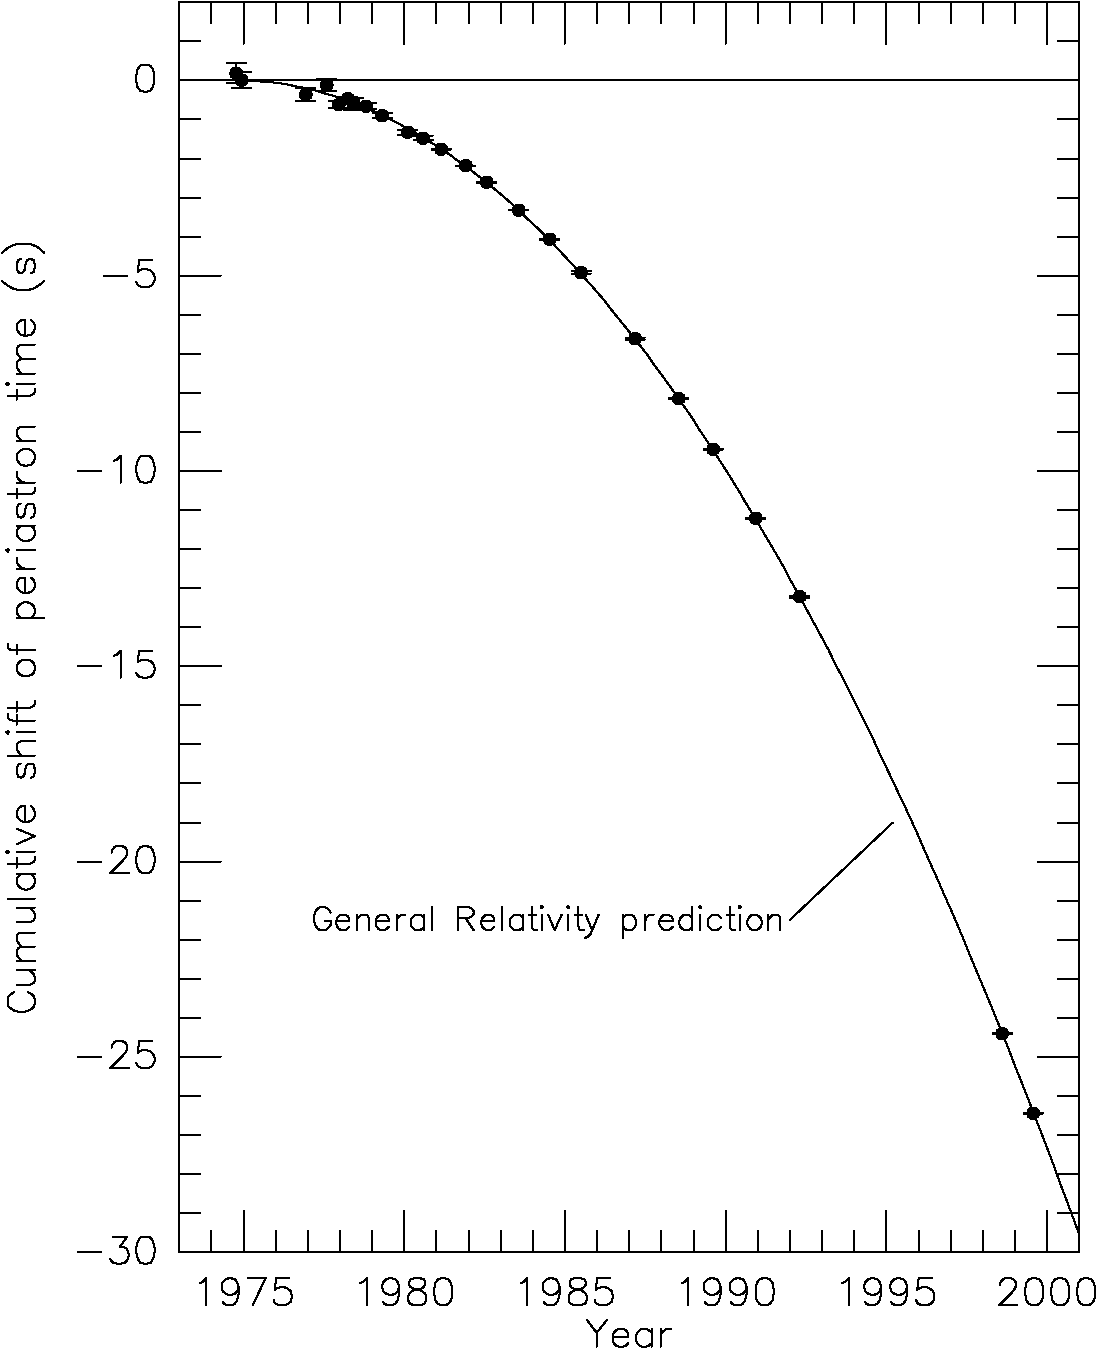
\includegraphics[width=0.45\textwidth]{figure/hulse-taylor-grav-wave}
  \caption{Andamento della precessione del periastro della pulsar binaria PSR
    1913+16 scoperta da Hulse e Taylor, fra il 1975 e il 2000.  Il buco negli
    anni '90 è dovuto alla chiusura del telescopio di Arecibo per aggiornamento.
    La linea continua rappresenta la predizione della relatività generale, che
    tiene conto dell'emissione di onde gravitazionali da parte della pulsar, con
    potenza dell'ordine \SI{e24}{\watt}.  Crediti:
    \textcite{2001LRR.....4....4W}}
  \label{fig:hulse-taylor-grav-wave}
\end{figure}
A circa \SI{7.3}{\kilo\parsec} di distanza da noi esiste un sistema binario
molto stretto costituito da due stelle di neutroni, di cui una è la pulsar PSR
B1913+16 (scoperta da Hulse e Taylor nel 1974), in orbita l'una attorno
all'altra con un periodo di $\simeq 8$ ore.  Le masse delle due stelle sono
$\simeq \SI{1.4}{\solarmass}$, la distanza fra le stelle è
$\simeq \SI{1.9e11}{\centi\metre} = \SI{1.9e6}{\kilo\metre}$ e la pulsar si
muove alla velocità di \SI{300}{\kilo\metre\per\second}.  Questo sistema è
importante perché fornisce una forte evidenza sperimentale, seppur indiretta,
della emissione di onde gravitazionali e della validità della Teoria della
Relatività Generale.  Grazie alle regolari emissioni di impulsi elettromagnetici
da parte delle pulsar, è stato possibile misurare i parametri orbitali del
sistema, in particolare la precessione del periastro del sistema (vedi
figura~\ref{fig:hulse-taylor-grav-wave}) e la dilatazione gravitazionale del
tempo (red-shift gravitazionale).

\subsection{Collasso gravitazionale}
\label{sec:collasso-grav}

Un'altra possibile sorgente di onde gravitazionali è il collasso gravitazionale
di un corpo massivo.  Poiché un processo di collasso sfericamente simmetrico,
per il teorema di Birkhoff, darebbe luogo a un campo statico, è necessario
ipotizzare che il corpo non sia dotato di simmetria sferica.  Un esempio di
questo fenomeno è quello di una stella che collassa in una stella di neutroni
(NS), visibile nel radio poi come pulsar.  La massa massima di una NS è di circa
qualche massa solare.  Approssimiamo la stella originaria con un ellissoide di
ellitticità $e$
\begin{equation}
  e = \frac{\text{differenza fra i raggi equatoriali}}{\text{raggio equatoriale
      medio}}  = \frac{a-b}{(a+b)/2} = 10^{-4},
\end{equation}
con raggi equatoriali $a$ e $b$ dell'ellissoide dell'ordine di $R_{0} \sim
\SI{7e5}{\kilo\metre}$.  Dopo il collasso la NS avrà dimensioni $R \simeq 10$ km
e a causa della conservazione del momento angolare $L \simeq M \omega R^2$,
ruoterà con velocità angolare $\omega \sim
\SI[per-mode=reciprocal]{e4}{\per\second}$ (si parla in questi casi di pulsar a
milli-secondi).  La potenza emessa dalla NS in rotazione sotto forma di onde
gravitazionali\footnote{Vedi \textcite[488]{shapiro:black-holes};
  \textcite[272]{weinberg:gravitation}.} è
\begin{equation}
  I_{\textup{og}} = \frac{32}{5} \frac{G}{c^{5}} \mathcal{I}^{2} \omega^{6}
  e^{2} \sim \SI{e47}{\erg\per\second}
\end{equation}
con $\mathcal{I} = \text{momento di inerzia} \sim MR^{2}$.  L'energia
rotazionale alla formazione della pulsar è
\begin{equation}
  E = \frac{1}{2} \mathcal{I} \omega^{2} \sim \SI{e53}{\erg}.
\end{equation}
Pertanto, se la luminosità $I_{\textup{og}}$ rimanesse costante nel tempo (in
particolare se l'eccentricità $e$ rimanesse costante), l'energia rotazionale
iniziale dovrebbe esaurirsi in un tempo $\var t = E/I$ dell'ordine di 1 anno,
cio\'e dopo un anno la stella dovrebbe smettere di ruotare.  In realtà noi oggi
osserviamo pulsar molto vecchie (la Crab è esplosa nel 1054).  Quindi siamo
costretti a ipotizzare che la NS dopo il collasso circolarizzi velocemente ($e
\to 0$) con la conseguente soppressione della potenza emessa in onde
gravitazionali.

Comunque, la stella di neutroni continua a emettere radiazione elettromagnetica
se è dotata di un momento di dipolo magnetico $\bm{m}$ non allineato con l'asse
di rotazione (modello di Pacini).

\section{Osservazione delle onde gravitazionali}
\label{sec:osservazione-onde}

\begin{figure}
  \centering
  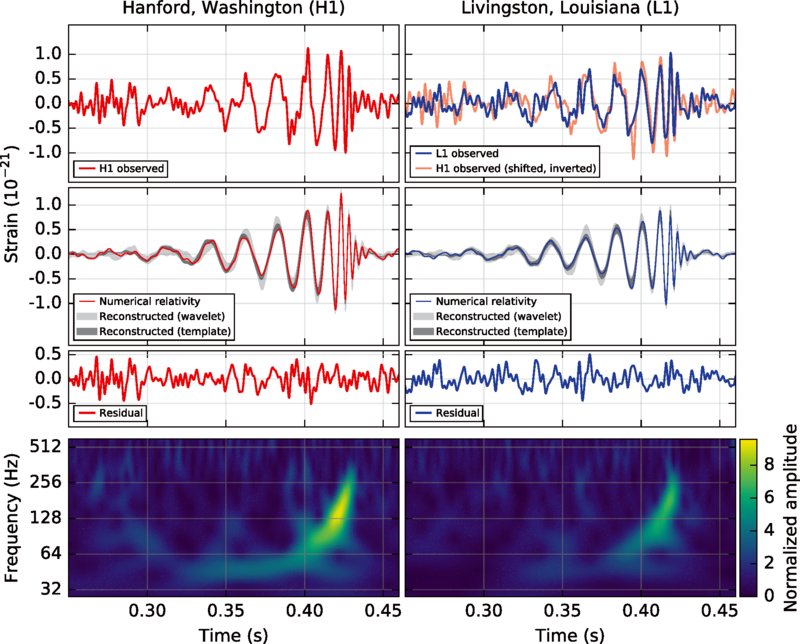
\includegraphics[width=0.7\textwidth]{figure/ligo-grav-wave-signal}
  \caption{Evento di onda gravitazionale GW150914, osservato da LIGO Hanford
    (sinistra) e Livingston (destra).  In alto: segnale registrato dai due
    interferometri.  Al centro: segnale ricostruito, con intervallo di
    confidenza del \(90\%\) usando due diversi modelli (in grigio) e modello
    teorico, derivante dalle relatività numerica, che meglio si adatta ai dati
    osservati (curve solide).  In basso: rappresentazione tempo-frequenza del
    segnale, che mostra la crescita della frequenza del segnale con il tempo}
  \label{fig:ligo-grav-wave}
\end{figure}
Il sistema binario di pulsar scoperto da Hulse e Taylor ha fornito la prima
prova indiretta delle onde gravitazionali, ma a 100 anni esatti dalla
pubblicazione della teoria della relatività generale, il 14 settembre 2015 i due
apparati interferometrici dell'esperimento LIGO hanno registrato il primo
segnale diretto di un'onda gravitazionale, riportato nella
figura~\ref{fig:ligo-grav-wave}, originatosi a \SI{410}{\mega\parsec} di
distanza dalla Terra.  L'onda è stata generata dal processo di fusione di due
buchi neri, rispettivamente di massa \SI{36}{\solarmass} e \SI{29}{\solarmass},
che hanno prodotto un buco nero finale di massa \SI{62}{\solarmass}.  Le \(3\)
masse solari mancanti alla somma aritmetiche delle masse individuali sono state
emesse sotto forma di onde gravitazionali nel tempo di \SI{0.2}{\second},
producendo una luminosità di onde gravitazionali di picco pari a
\SI{3.6e56}{\erg\per\second}
(\(=\SI{200}{\solarmass\clight\squared\per\second}\)).  La sorgente di onde di
questo evento è stata dunque un sistema binario, come quello descritto nel
paragrafo~\ref{sec:sistema-binario}.

Questa scoperta è stata molto importante per l'astrofisica perché, oltre a
osservare direttamente per la prima volta le onde gravitazionali, ha fornito
un'ulteriore prova a sostegno dell'esistenza dei buchi neri di massa stellare,
in particolare più massivi di \SI{25}{\solarmass}, e che essi possono costituire
dei sistemi binari di buchi neri che possono poi fondersi in tempi minori
rispetto al tempo di Hubble.

Il segnale è giunto al rivelatore di Hanford, che si trova più a nord, con
\SI{6.9}{\milli\second} di ritardo rispetto a Livingston, indicando che l'onda
proveniva da qualche parte nell'emisfero meridionale.  Dato che solo questi due
rivelatori erano attivi durante l'evento,\footnote{L'esperimento italo-francese
  Virgo, con sede a Càscina (Pisa, Italia) era in fase di ampliamento per
  aumentarne la sensibilità.} non è stato possibile determinare con maggiore
precisione la direzione della sorgente di onde.

\begin{figure}
  \centering
  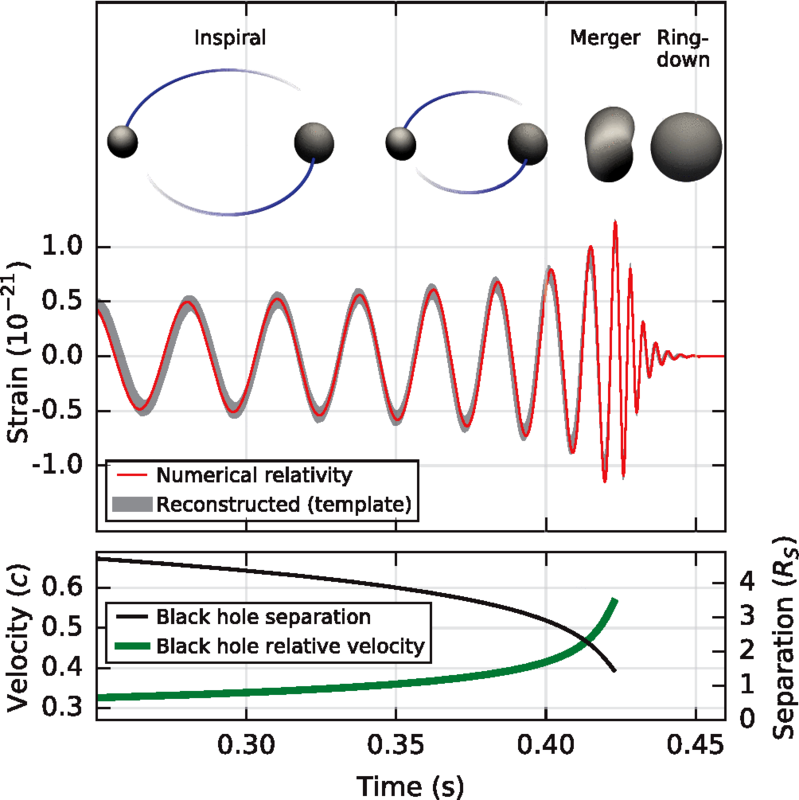
\includegraphics[width=0.7\textwidth]{figure/ligo-estim-strain}
  \caption{Ricostruzione dell'evento di onda gravitazionale GW150914.  In alto:
    rappresentazione artistica dell'evento, secondo i modelli di relatività
    numerica.  Al centro: ampiezza stimata del segnale dell'onda gravitazionale.
    In basso: andamento della separazione dei due buchi neri e della loro
    velocità relativa}
  \label{fig:ligo-strain}
\end{figure}
Nella figura~\ref{fig:ligo-strain} è mostrata la ricostruzione dell'evento.  La
fase della loro fusione vera e propria (\emph{merger}) è stata preceduta da un
loro spiraleggiamento (\emph{inspiral}) dei due buchi neri l'uno attorno
all'altro e seguita dallo smorzamento del segnale (\emph{ring-down to Kerr}) una
volta che si è formato un nuovo buco nero di Kerr.  Dalla analisi delle
frequenze delle onde, riportate nella figura~\ref{fig:ligo-grav-wave}, si è
trovato che nell'arco dei \SI{0.2}{\second} di durata dell'evento le frequenze
sono andate da \num{30} a \SI{150}{\hertz} e la massa chirp per questo evento è
risultata pari a \(\mathcal{M} \simeq \SI{30}{\solarmass}\).  Attraverso un
ulteriore processo di fit a modelli numerica è stato possibile stimare le masse
individuali dei due buchi neri riportate all'inizio di questo paragrafo.

%%% Local Variables:
%%% mode: latex
%%% TeX-master: "../gravitazione"
%%% fill-column: 80
%%% End:
